\documentclass[a4paper,oneside,12pt]{report}
\setlength\textwidth{155mm}
\setlength\textheight{247mm}
\setlength\topmargin{-10mm}
\setlength\headheight{15pt} % Pro zbavení se warningů
\setlength\oddsidemargin{05mm}
\setlength\evensidemargin{05mm}
\let\openright=\clearpage


%% Vytváříme PDF/A-2u
\usepackage[a-2u]{pdfx}

%% Přepneme na českou sazbu a fonty Latin Modern
\usepackage[czech]{babel}
\usepackage[utf8]{inputenc}
\usepackage{lmodern}
\usepackage[T1]{fontenc}
\usepackage{textcomp}

\usepackage{subcaption,wrapfig} % pro použití subfigure
\usepackage{amsmath}						% rozšíření pro sazbu matematiky
\usepackage{amsfonts}						% matematické fonty
\usepackage{amsthm}							% sazba vět, definic apod.
\usepackage{bbding}							% balíček s nejrůznějšími symboly (čtverečky, hvězdičky, tužtičky, nůžtičky, ...)
\usepackage{bm}									% tučné symboly (příkaz \bm)
\usepackage{graphicx}						% vkládání obrázků
\usepackage{fancyhdr}						% možnost stylizovat záhlaví
\usepackage{fancyvrb}						% vylepšené prostředí pro strojové písmo
\usepackage{indentfirst}				% zavede odsazení 1. odstavce kapitoly
\usepackage[nottoc]{tocbibind} 	% zajistí přidání seznamu literatury,
\usepackage{icomma}         		% inteligentní čárka v matematickém módu
\usepackage{dcolumn}        		% lepší zarovnání sloupců v tabulkách
\usepackage{booktabs}       		% lepší vodorovné linky v tabulkách
\usepackage{paralist}       		% lepší enumerate a itemize
\usepackage{caption}						%	popisky
\usepackage{dirtree}						% strom souborů
\usepackage{minted} 						% vkládání kódu
\usepackage[bottom]{footmisc}  	% poznámky pod čarou vespod
\usepackage{bibentry} 					% citace přes celé heslo, používáno u první citace z jednoho zdroje
\usepackage{xurl}								% umožní url zalomit všude
\usepackage{hyperref} 					% odstranění červených okrajů v obsahu
\usepackage{enumitem}
\nobibliography*

\usepackage{color}
\usepackage{natbib}

\definecolor{pblue}{rgb}{0.13,0.13,1}
\definecolor{pgreen}{rgb}{0,0.5,0}
\definecolor{pred}{rgb}{0.9,0,0}
\definecolor{pgrey}{rgb}{0.46,0.45,0.48}
\renewcommand{\baselinestretch}{1.2}
\setlist[itemize]{nosep,itemsep=1mm,topsep=-0.5em}
\def\labelitemi{--}
%%% Údaje o práci

\def\NazevSkoly{Gymnázium, Praha 6, Arabská 14}
\def\TypPrace{Ročníkový projekt}
% Název oboru i se slovem 'obor/předmět'
\def\NazevOboru{obor Programování}
\def\NazevPrace{Bazar Učebnic Arabská}
\def\NazevPraceShort{BookExchange}
\def\AutorPrace{Josef Litoš}
\def\Trida{4. E}
\def\VedouciPrace{Ing. Daniel Kahoun}
\def\DatumOdevzdani{únor 2022}

% Anotace (doporučený rozsah cca 80-200 slov; podrobnější popis práce)
\def\Anotace{
	Tento projekt si klade za cíl vytvořit stránku, na které budou moci studenti inzerovat
	své učebnice, které již nepotřebují, a žáci nižších ročníků si je tak budou moci
	pořídit. O průběhu obchodu jsou uživatelé informováni prostřednictvím emailu, kterým se
	přes Google OAuth přihlásí. Na email dostanete všechna upozornění týkající se hledané
	knihy, příchozích požadavků, nebo změn některých z objednávek. Buď knihu dostanete Vy,
	nebo někdo jiný. V každém případě se o jejím	prodání dozvíte.
}
\def\AnotaceEN{
	This project sets as a goal to create a page, on which students will be able to post
	their textbooks they are not in need of. Pupils of lower classes can then buy them.
	Users are informed about the current state of their trade through email that they will
	use in Google OAuth to log in. In fact, you will receive all notifications on your email
	being it a new book you were looking for, a new incoming request or a change in
	requests of your own. Either the book goes to you or to someone else. Both ways, you
	will know, when the book was sold.
}
\def\AnotaceDE{
	Dieses Projekt stellt sich vor, eine Seite zu machen, auf welcher Studenten ihre nicht
	mehr benutzte Lehrbücher anzeigen können. Schüler aus unteren Studienjahren können sich
	diese Anzeige ansehen und die Bücher kaufen. Benutzer werden über den Status des Handels
	per Email informiert. Die gleiche Email wird auch bei der Google OAuth Anmeldung benutzt.
	Ihre Email bekommt alle Hinweisen, soll das ein neues Buch, das Sie gesucht haben, neues
	Gesuch, oder eine Veränderung in Ihre Anträgen sein. Entweder geht das Buch zu Ihnen,
	oder zu jemandem anderen. In beiden Varianten werden Sie über seine Verkauf informiert.
}

% 3 až 5 klíčových slov (doporučeno), každé uzavřeno ve složených závorkách
\def\KlicovaSlova{
	React, Node, SQL, OAuth
}

\def\Zadani{%
	Vytvořte webovou aplikaci, která umožní uživateli následující
	\begin{itemize}
		\item reagovat na inzerovanou knihu
		\item zobrazit a filtrovat dostupné knihy
		\item přihlásit se o knihu, jakmile bude dostupná
		\item automatizované odstranění inzerátu po zakoupení
		\item přidat, odstranit a upravit vlastní inzeráty (včetně fotky)
	\end{itemize}
}
\def\Bonus{%
	\begin{itemize}
		\item vlastní verze UI pro mobilní zařízení
		\item nabídka balíčku knih s výhodnější cenou
		\item administrátorský přístup do databází z webu
		\item integrace chatu pro domluvu na předání mezi uživateli
	\end{itemize}
}

%% Balíček hyperref, kterým jdou vyrábět klikací odkazy v PDF,
%% ale hlavně ho používáme k uložení metadat do PDF (včetně obsahu).
\hypersetup{unicode}
\hypersetup{breaklinks=true}
\hypersetup{pdfborder=0 0 0}

%% Definice různých užitečných maker (viz popis uvnitř souboru)
%%% Tento soubor obsahuje definice různých užitečných maker a prostředí %%%
%%% Další makra připisujte sem, ať nepřekáží v ostatních souborech.     %%%

%%% Drobné úpravy stylu

% Tato makra přesvědčují mírně ošklivým trikem LaTeX, aby hlavičky kapitol
% sázel příčetněji a nevynechával nad nimi spoustu místa. Směle ignorujte.
\makeatletter
\def\@makechapterhead#1{
	{\parindent \z@ \raggedright \normalfont
		\Huge\bfseries \thechapter. #1
		\par\nobreak
		\vskip 20\p@
	}}
\def\@makeschapterhead#1{
	{\parindent \z@ \raggedright \normalfont
		\Huge\bfseries #1
		\par\nobreak
		\vskip 20\p@
	}}
\makeatother

% Toto makro definuje kapitolu, která není očíslovaná, ale je uvedena v obsahu.
\def\chapwithtoc#1{
	\chapter*{#1}
	\addcontentsline{toc}{chapter}{#1}
}

% Trochu volnější nastavení dělení slov, než je default.
\lefthyphenmin=2
\righthyphenmin=2

% Zapne černé "slimáky" na koncích řádků, které přetekly, abychom si
% jich lépe všimli.
\overfullrule=1mm

%%% Makra pro definice, věty, tvrzení, příklady, ... (vyžaduje baliček amsthm)

\theoremstyle{plain}
\newtheorem{veta}{Věta}
\newtheorem{lemma}[veta]{Lemma}
\newtheorem{tvrz}[veta]{Tvrzení}

\theoremstyle{plain}
\newtheorem{definice}{Definice}

\theoremstyle{remark}
\newtheorem*{dusl}{Důsledek}
\newtheorem*{pozn}{Poznámka}
\newtheorem*{prikl}{Příklad}

%%% Prostředí pro důkazy

\newenvironment{dukaz}{
	\par\medskip\noindent
	\textit{Důkaz}.
}{
	\newline
	\rightline{$\square$}  % nebo \SquareCastShadowBottomRight z balíčku bbding
}

%%% Prostředí pro sazbu kódu, případně vstupu/výstupu počítačových
%%% programů. (Vyžaduje balíček fancyvrb -- fancy verbatim.)

\DefineVerbatimEnvironment{code}{Verbatim}{fontsize=\small, frame=single}

%%% Prostor reálných, resp. přirozených čísel
\newcommand{\R}{\mathbb{R}}
\newcommand{\N}{\mathbb{N}}

%%% Užitečné operátory pro statistiku a pravděpodobnost
\DeclareMathOperator{\pr}{\textsf{P}}
\DeclareMathOperator{\E}{\textsf{E}\,}
\DeclareMathOperator{\var}{\textrm{var}}
\DeclareMathOperator{\sd}{\textrm{sd}}

%%% Příkaz pro transpozici vektoru/matice
\newcommand{\T}[1]{#1^\top}

%%% Vychytávky pro matematiku
\newcommand{\goto}{\rightarrow}
\newcommand{\gotop}{\stackrel{P}{\longrightarrow}}
\newcommand{\maon}[1]{o(n^{#1})}
\newcommand{\abs}[1]{\left|{#1}\right|}
\newcommand{\dint}{\int_0^\tau\!\!\int_0^\tau}
\newcommand{\isqr}[1]{\frac{1}{\sqrt{#1}}}

%%% Vychytávky pro tabulky
\newcommand{\pulrad}[1]{\raisebox{1.5ex}[0pt]{#1}}
\newcommand{\mc}[1]{\multicolumn{1}{c}{#1}}


%% Titulní strana a různé povinné informační strany
\fancypagestyle{plain}{
\fancyhf{}
% \renewcommand{\headrulewidth}{0.4pt}
\renewcommand{\footrulewidth}{0.4pt}
\fancyhead[L]{{\TypPrace} -- \NazevSkoly}
\fancyhead[C]{}
\fancyhead[R]{}
\fancyfoot[L]{\AutorPrace, \Trida}
\fancyfoot[C]{\NazevPraceShort}
\fancyfoot[R]{\thepage}
}


\begin{document}

%%% Titulní strana práce
\pagestyle{empty}
\hypersetup{pageanchor=false}

\begin{center}
	\begin{figure}[h!]
		\begin{center}
			\begin{subfigure}[b]{0.1\linewidth}
				\def\svgwidth{\columnwidth}\scalebox{1}{\input{../img/logo.pdf_tex}}
			\end{subfigure}
			\begin{subfigure}[b]{0.8\linewidth}
				{\LARGE\bfseries\NazevSkoly}

				\vspace{3mm}

				{\LARGE\TypPrace, \NazevOboru}
				\vspace{-1mm}
			\end{subfigure}
		\end{center}
	\end{figure}

	\vfill

	\def\svgwidth{\columnwidth}\scalebox{0.3}{\input{../img/BElogo.pdf_tex}}

	\vfill

	{\bf\Huge\NazevPraceShort}

	\vspace{3.5mm}
	{\bf\Large\NazevPrace}

	\vfill
	\vfill

	Vypracoval: \hfill \AutorPrace

	Vedoucí práce: \hfill \VedouciPrace

	\vspace{5mm}
	\DatumOdevzdani
\end{center}

\newpage
\hypersetup{pageanchor=true}
\pagestyle{plain}
\pagenumbering{arabic}

\openright

\vspace*{\fill}

\noindent
\textit{
	Prohlašuji, že jsem jediným autorem této práce, všechny citace jsou řádně označené
	a všechna použitá literatura a další zdroje jsou v práci uvedené. Tímto dle zákona
	121/2000 Sb. (tzv. Autorský zákon) ve znění pozdějších předpisů uděluji bezúplatně škole
	Gymnázium, Praha 6, Arabská 14 oprávnění k výkonu práva na rozmnožování díla (§ 13) a
	práva na sdělování díla veřejnosti (§ 18) na dobu časově neomezenou a\,bez omezení
	územního rozsahu.
}

\vspace{1cm}

\noindent
V .............. dne .............. \hfill Podpis autora .............................

\newpage

\openright

\vbox to 0.20\vsize{
	\setlength\parindent{0mm}
	\setlength\parskip{5mm}

	{\bf Anotace:} \Anotace

	{\bf Abstract:} \AnotaceEN

	{\bf Abstrakt:} \AnotaceDE

	{\bf Klíčová slova / Keywords / Schlüsswörter:} \KlicovaSlova

	{\bf Zadání:} \Zadani
	\vspace{1em}
	{\bf Bonusové funkce:} \Bonus

	\vss
}

\newpage

\openright



\tableofcontents

\chapter*{Úvod}
\addcontentsline{toc}{chapter}{Úvod}
Na začátek bych rád vysvětlil své myšlenkové pochody, kterými jsem byl doveden k tematu
této práce, a proč mi přijde tato aplikace vcelku užitečná.

Již po dva celé roky ovlivňuje probíhající pandemie fungování takřka všech státních i
soukromnických aparátů. Kromě globálně známých problémů to způsobilo i mnoho lokálních
potíží obzvlášť znatelných v dobách lockdownu. Příklady toho jsou častější rodinné spory,
často zrušení sportovních kroužků, a pro tento text nejpodstatnější -- zrušení konání
burzy učebnic.

Jelikož z předešlých let se učebnice hromadily, a burza učebnic byla tou nejrychlejší,
nejsnazší a často také nejvýhodnější cestou, jak učebnice vyřadit, jejich uskladňování
nebylo ideálním řešením. V tu dobu ale žádná náhrada podobného stylu za školní burzu
nebyla. Tím pádem se jevil jasný nápad -- udělat si vlastní burzu a dát ji na stránky
školy.

\vspace{1em}
Dokumentace je rozdělena na tři celky uvedené v pořadí nástavby programu. Každý z celků
projednává svou funkci v programu, vnitřní rozdělení, vzájemné vztahy a problémy s danou
částí spojené.


\chapter{Databáze}
\begin{wrapfigure}{r}{7.8cm}
	\vspace{-2.5mm}
	\def\svgwidth{\columnwidth}\scalebox{0.5}{\input{../img/ER_Diagram.pdf_tex}}
	\caption{\textit{Diagram používané databáze}}\label{fig:ER_Diagram}
\end{wrapfigure}

Chceme-li pracovat s daty a nějak je ukládat, je pravděpodobné, že se rozhodneme použít
nějakou databázovou strukturu. V případě tohoto programu je využíváno prostředí SQL běžící
na serveru MariaDB.

SQL má několik svých výhod a vhodných využití, pro které bylo zvoleno pro použití v tomto
programu. Mezi ně patří vhodnost pro jednoduchá data (myšleno ne objekty), spolehlivost a
uzpůsobení pro velká množství dat. Jiné databáze, jako třeba MongoDB, jsou vhodnější pro
ukládání celých objektů, čehož tento projekt nevyužívá.

\section{Uživatel}
Tabulka uživatelů je naprosto základním prvkem, od kterého se veškeré dění dále odvíjí.
Všechny ostatní tabulky se na ni odkazují. Pro vytvoření knihy musíme mít jasno v tom, kdo
knihu přidal, a kdo o ní žádá. Každý uživatel by dále pravděpodobně rád viděl jasný znak,
že je přihlášen, proto se ukládá i odkaz na jeho profilovou fotku, která se mu zobrazí po
přihlášení do stránky.

V obrázku \ref{fig:ER_Diagram} v tabulce \texttt{user} můžeme vidět, že si
program také udržuje přehled o\,\,posledním příhlášení uživatele, aby mohl v případě
dlouhodobé neaktivity informovat o možném smazání účtu z důvodu neaktivity. Je to snadný a
zároveň efektivní způsob, jak systém čistit od nejspíše již nepooužívaných dat.

Uložení přihlašovacích údajů přineslo malý problém -- zdá se, že \texttt{id}
nelze uložit jako číslo o délce 23 číslic. Ať už se vytvoří sloupec dlouhý 32 číslic, nebo
ne, SQL server v obou případech tvrdil, že je číslo příliš velké. Použití typu
\texttt{BIGINT} situaci nijak nezměnilo. Kvůli tomuto zatím nevysvětlenému úkazu
bylo třeba uložit číslo jak text (v SQL terminologii toto představuje typ
\texttt{VARCHAR}).

\newpage
\section{Kniha}
Tabulka knihy (v diagramu označeno jako \texttt{'book'}) představuje obecný vzor
pro jakýkoli inzerát. Předpokládá se, že budou přidávány převážně učebnice, případně
pracovní sešity, pro něž je tento termín také odpovídající.

Aby se každý hledající mohl ujistit, že našel, co hledal, vyžaduje každý inzerát název,
autora i rok vydání. Samozřejmostí je pak cena, která je úmyslně omezena do 1000 Kč, neboť
lze předpokládat, že žádný učební materiál jako jeden kus nebude přesahovat tuto cenu.

Už v průběhu testování se ukázalo 64 znaků pro název jako nedostatečné. Dvojnásobek se
ukázal jako přijatelné množství kromě jména také pro autory, kteří nejspíše nebudou tolik
ověřováni, čímž pádem bylo možné využít kratší délky a počítat s možností, že inzerenti
budou muset upustit tituly autorů, pokud jich bude více než 2.

Popisek je čistě dobrovolným polem s cílem poskytnou příležitost sdělit hledajícím určité
další informace, které třeba nebyly vhodné do žádné jiné položky. Příkladem může být
informace o popsání knihy nebo také přímo přidaná informace, kde se pro knihu stavit, jako
kupříkladu do které třídy jít za majitelem. Byť je komunikace možná přes email, někteří
mohou preferovat pokus o co nejpřímější a nejrychlejší způsob komunikace.

\section{Žádost}
Když objevíme knihu, kterou bychom si rádi pořídili, musíme si o ni zažádat. Všechny tyto
žádanky se ukládají do tabulky \texttt{request}, kde uchováváme odkaz na žádajícího
a knihu, o kterou žádá. Majitel knihy může přijmout pouze jednu žádost (stav přijmutí je
zaznamenán ve sloupci \texttt{accepted}), může žádosti na svou knihu také rušit.
Zrušit své rozhodnutí může samozřejmě také žadatel.

\section{Upozornění}
Upozornění (v tabulce \texttt{notification}) obvykle obsahují text k zaslání a jsou
odeslána ihned. V tomto případě se jedná o princip lehce odlišný.

Název pro tento seznam se může zdát být poněkud matoucí, jedná se však o uložený text,
který uživatel, uvedený v upozornění, hledal v naději nalézt knihu. Pokud ale hledanému
výrazu žádná kniha neodpovídá, je možné zažádat si o upozornění na přidání hledané knihy,
čímž se myslí kniha, jejíž název obsahuje hledaný text.


\chapter{Server}
Všechny mechanismy a požadavky jsou zpracovávány na severu. Když uživatel chce cokoli
provést, stačí zavolat správnou cestu a předat potřebná data pro dokončení akce. Server
požadavek zpracuje, zapíše potřebná data do databáze a, pokud to situace vyžaduje, zašle
příslušné osobě informativní email.

\section{Autentifikace}
Pro většinu úkonů je ale potřeba být přihlášen, na to je využíván middleware
\texttt{passport}, který proces autentifikace značně zjednodušuje. Na ověření nám
stačí \texttt{id} uživatele a email, protože autentifikaci k účtu jako takovému
za nás řeší Google OAuth. Tento přístup je pohodlnější i pro zákazníky, jelikož nemusejí
vytvářet žádný nový účet a stačí jim použít už vytvořený školní účet, který je také
propojený s Googlem.

Identifikátor a email jsou ukládané v cookie prohlížeče a při přihlášení se vždy doplní o
obrázek a jméno uživatele, třebaže jeho jméno není momentálně nijak využíváno. Pro
pozdější komunikaci uvnitř aplikace by pak už bylo vhodné, aby uživatelé věděli, jak se
navzájem oslovit. Proto ukládáme i zobrazované jméno.

\section{Vstup do databáze}
Na připojení k databázi je využito návrhového vzoru tovární metody
(\texttt{sql.js create()}), která před vrácením metody pro zadávání příkazů databázi nejprve
ověří, zda obalovou metodu k dané databázi již nevytvořila a případně ji vrátí.

Tento způsob přistupování je obecně napsaný, ale byť tato aplikace využívá pouze jednu
databázi (jmenovitě \texttt{book{\_}exchange}), člověk nikdy neví, kdy mu trocha flexibility
navíc přijde vhod.

Všechny tabulky mají své fasády ve složce \texttt{services} jako soubory, které
přístup do databáze dále zjednodušují svými metodami na přidání, odebrání, a zpracovávají
všechny další funkce, které se s jednotlivými tabulkami pojí (např. vyhledávání knih).

\section{Přístupové body}
Všechny endpointy pro komunikaci se serverem mají prefix \texttt{/api}. Každá
akce, která potřebuje získat nějaká data pro vykreslení stránky, přistupuje k nějaké cestě
a tvoří požadavky. Tato kapitola tyto cesty, jejichž rozřazování řeší patřičné soubory pod
složkou \texttt{routes} (\texttt{user.js} pro cesty \texttt{/api/user}
atd.), uvede a vystvětlí práci prováděnou při jejich zavolání;
všechny dále zmíněné soubory nalezneme ve složce \texttt{services}.

\subsection{\texttt{/user}}
\begin{wrapfigure}[8]{r}{4cm}
	\vspace{-6.5mm}
	\caption{\textit{dostupné cesty pro \texttt{/user}}}\label{fig:/user}
	\vspace{-7mm}
	\begin{minted}[gobble=1]{yaml}
	/login: #GET
	/gcallback: #GET
	/info: #GET
	/logout: #GET
	/: #DELETE
	/books: #GET
  \end{minted}
\end{wrapfigure}

Základní akcí pro fungování aplikace je přihlášení (\texttt{/login}, viz obrázek
\ref{fig:/user}), ze kterého jsme přesměrováni \texttt{passport}em na
přihlašovací stránku Google, která nám vrátí potřebné údaje pro přihlášení na cestu
\texttt{/gcallback}. Zbytek práce se provádí, stejně jako u většiny ostatních cest, ve
stejnojmenné metodě jako je cesta (\texttt{login()}) v souboru názvu příslušné
tabulky, s\,\,níž pracujeme (\texttt{user.js}).

Pokud se jedná o registraci, tedy uživatel není nalezen v\,\,databázi, je nový učet do
databáze automaticky přidán. Tím pádem není zapotřebí oddělovat registraci a přihlášení a
můžeme uživatele nového i stávajícího přihlásit stejným způsobem, který zahrnuje u
aktualizaci jména, či profilového obrázku, pokud by je náhodou od své poslední návštěvy
změnil.

Pokud už je uživatel přihlášen (tzn. má cookie se svým emailem a id), pak pro získání
všech dat spojených se svým účtem přistupuje k cestě \texttt{/info}, která jen
vrátí záznam účtu z databáze.

Cesta \texttt{/logout} řeší odhlášení uživatele, kdy dochází k smazání cookie z
příchozího požadavku, což efektivně odstraní z prohlížeče všechna data o uživateli.

Zavoláme-li samotnou cestu \texttt{/api/user/} metodou \texttt{DELETE}, server
náš účet z databáze smaže, čímž se smažou i všechny inzeráty a žádosti s nimi, nebo s
námi, spojené. Nakonec se vyčistí i cookie z requestu, aby nedocházelo k chybě, kdy se
zákazník snaží přihlásit se starými údaji, které již v databázi nejsou.

Poslední adresou je získání všech inzerovaných položek -- \texttt{/books}. Tento
bod příjímá také parametr \texttt{q} představující vyhledávaný výraz, podle
kterého máme knihy vybrat.

\subsection{\texttt{/book}}
\begin{wrapfigure}[8]{r}{4.2cm}
	\vspace{-6.5mm}
	\caption{\textit{dostupné cesty pro \texttt{/book}}}\label{fig:/book}
	\vspace{-6.5mm}
	\begin{minted}[gobble=1]{yaml}
	/: #POST
	/$id: #PATCH
	../books: #GET
	/$id: #GET
	/$id/edit: #GET
	/$id: #DELETE
	/$id/requests: #GET
  \end{minted}
\end{wrapfigure}

Tato aplikace je o knihách, není těžké si domyslet, že se s\,nimi bude také nejvíce
pracovat (viz obrázek \ref{fig:/book}). Bohužel se při práci objevily jisté
problémy, kvůli kterým se musely dělat kličky.

\subsubsection{Manipulace s knihou}
Prvním krokem, je knihu přidat (\texttt{/ \#POST}). Zde se neděje nic zajímavého.
Když je uživatel přihlášen a předal všechna data potřebná k vytvoření knihy včetně
náhledové fotky, tak knihu vytvoříme a fotku uložíme jako JPG obrázek s patřičným id.
Stejný příběh je i u úpravy knihy (\texttt{/\$id \#PATCH}) -- obdržíme všechna data,
zjistíme, co je třeba pozměnit a\,\,inzerát aktualizujeme, samozřejmě úpravu může provést
pouze z účtu knihu inzerující. Finálně můžeme po provedení obchodu knihu smazat
(\texttt{/\$id \#DELETE}).

\subsubsection{Data fetching}
Pro získávání dat o knihách jsou k dispozici tři cesty, ale nejvíce bude v užitku adresa
\texttt{/api/books} vracející všechny knihy, nebo knihy odpovídající hledanému výrazu
\texttt{q}.

Druhá možnost je zeptat se na data knihy přímo, na to už je potřeba znát její id.

Konečně třetí možnost (\texttt{/\$id/edit}), byť by svým názvem spíš naváděla k
domněnce, že sem zasíláme upravené knihy, vrací stejná data, jako dotaz na jednu knihu.
Rozdíl spočívá v kontrole, jež kontroluje právo uživatele knihu upravit.

Ačkoli se zdá, že bychom mohli kontrolu autorství provádět u klienta a není třeba na to
vytvářet oddělený endpoint, v procesu vytváření frontendu se ukázala práce s\,\,uživatelem
jako nemožná, přinejmenším v této části programu. Přesněji řečeno globální stav aplikace
vždy při prvním zavolání vrátí prázdnou hodnotu a po získání dat o\,\,uživateli již (z
nepochopitelného a nezjištěného důvodu) odmítá stránku na úpravu knížky aktualizovat,
takže není způsob, jak zjistit, jestli je uživatel přihlášen.

\vspace{1em}
Poslední endpoint \texttt{/\$id/requests} oproti předešlým nevrací knihy, jak by se dalo
očekávat, nýbrž všechny žádanky o danou knihu. Další operace s žádostmi jsou popsány níže.

\subsection{\texttt{/request}}
\begin{wrapfigure}[9]{r}{4.2cm}
	\vspace{-6.5mm}
	\caption{\textit{dostupné cesty pro \texttt{/requests}}}\label{fig:/request}
	\vspace{-6.5mm}
	\begin{minted}[gobble=1]{yaml}
	/: #POST
	/$id/accept: #PATCH
	/$id: #DELETE
	/$id/abort: #POST
	/forMe: #GET
	/fromMe: #GET
  \end{minted}
\end{wrapfigure}


Reakce na cizí inzerát je reprezentována vytvořením nového záznamu do tabulky
\texttt{request}. Všechny cesty vyobrazené v obrázku \ref{fig:/request} zde
dále vysvětlíme do potřebné hloubky.

Přidání neskrývá žádné změny. Pošleme číslo knihy jako parametr \texttt{book{\_}id} a
žádost propojující zákazníka s knihou se hned vytvoří spolu s emailem odeslaným majiteli
knihy, aby věděl, že se někdo o jeho knihu zajímá. Více o zasílání emailů v následující
kapitole \ref{chap:/mails}.

Vlastník má navíc právo žádost přijmout (\texttt{/\$id/accept}), což mu zpřístupní
informace o kontaktu, přesněji jméno a email, na zákazníka, které obdrží mailem. Do té
doby mají z anonymizačních důvodů přístup pouze ke svým knihám a zobrazení všech s nimi
spojených žádostí, z nichž je publikováno pouze číslo žádosti a cílené knihy.

Odstranění má dvě podoby. Majitel knihy může žádost zamítnout a přímo ji smazat
(\texttt{/\$id \#DELETE}) a žadatel zrušit (\texttt{/\$id/abort}). Cílové cesty jsou
rozdělené pro přehlednost kódu a snazší ověření oprávnění k provedení akce.

Poslední dvě adresy vrátí seznam žádostí, které se vztahují k Vám. Žádosti
\texttt{/forMe} představují příchozí odpovědi na Vaše inzeráty. Oproti tomu
\texttt{/fromMe} zobrazí Vámi odeslané žádosti na knihy uživatelů ostatních.

\subsection{\texttt{/notify}}

Endpoint \texttt{/api/notify} je výjimkou v mnoha ohledech. Nemá další podvětev a je
registrován hlavním souborem serveru (\texttt{app.js}), neboť je zbytečné pro
jediný přístupový bod vytvářet celý vlastní soubor, když nění nijak komplexní na
zpracování.

Tato adresa je volána v případech, kdy zákazník nenalezl žádnou knihu pro hledaný výraz,
ale rád by obdržel upozornění o přidání knihy, která by onomu řetězci odpovídala. O to se
opět postará soubor pracující s příslušnou tabulkou (\texttt{notification})
a\,\,upomínku zapíše.

Tento systém spoléhá na solidaritu uživatelů, a tedy, že nebudou vytvářet upomínky na
velká množství nesmyslných názvů, které se nejspíš ve výběru nikdy neobjeví. V\,\,takové
situaci by každé přidání knihy, jak bylo popsáno výše, utržilo velké časové penále
způsobené kontrolou všech upomínek.

\section{Zasílání emailů}\label{chap:/mails}
\begin{wrapfigure}{r}{5.9cm}
	\vspace{-4mm}
	
\includegraphics{../img/mail.png}
	\caption{\textit{email obdržený po přijetí žádosti}}\label{fig:mail}
\end{wrapfigure}

Všechny změny týkající se žádostí se vždy vztahují k dalšímu účtu, který je třeba
informovat o\,\,změně. V současné chvíli pro emailování stačí jediná šablona, u které není
třeba víc, než měnit titulek, podrobnější popisek a odkaz tlačítka zobrazeného pod kartou
knížky v jednání. Šablona je zpracovávána frameworkem \texttt{handlebars} určeným pro
design emailů, které se odesílají přes plugin \texttt{nodemailer}. Podobu šablony při
použití je možno vidět na obrázku \ref{fig:mail}.

Majitel knihy obdrží zprávu pokud:
\begin{itemize}
	\setlength\itemsep{0em}
	\item obdržel žádost o nabízenou knihu
	\item žadatel už o jeho knihu nestojí
	\item přijal nabídku
\end{itemize}

\vspace{1em}
Žádající o knihu je informován o:
\begin{itemize}
	\setlength\itemsep{0em}
	\item zrušení jeho žádosti
	\item zmizení knihy z trhu
	\item přijetí zaslané nabídku
	\item nalezení jím hledané knihy
\end{itemize}

\vspace{1em}
Pro zprávy odeslané po přijetí žádanky oběma účastníkům obchodu je navíc vygenerován
výchozí text mailu na první zkontaktování protější strany.


\chapter{Webová stránka}
V Předešlé části jsme se zaměřili na propojení stránky s databází za pomoci backendu,
který da nás provádí všechnu prácí. Díky tomu stačí na každou akci dát pokyn na patřičnou
adresu a všechno se za nás zpracuje. Přesto většina problému teprve přijde, totiž práce s
Reactem je, jak známo, jednoduchá na započetí, ale náročná na správné provedení.

\section{Záhlaví}
\begin{wrapfigure}[3]{r}{5cm}
	\vspace{-5mm}
	\centering
	
\includegraphics{../img/Header.png}
	\vspace{-2mm}
	\caption{\textit{záhlaví stránky}}\label{fig:header}
\end{wrapfigure}

Záhlaví je přítomné ve všech cestách stránky. Máme zde k dispozici odkaz na hlavní
stránku, vyhledávací pole a tlačítko uživatele, v jehož menu nalezneme možnosti přidání
knihy, zobrazení profilu a odhlášení -- za předpokladu, že je uživatel přihlášen. Jinak
uvidíme ikonku účtu bez profilu, která nás nabádá k přihlášení (viz obr.
\ref{fig:header}).

S designem aplikace nám ve všech částech pomáhá knihovna MaterialUI, která poskytuje již
nastylované komponenty, které můžeme rovnou zobrazit a nestarat se o css. Příkladem je ono
vyhledávací pole, které se automaticky přizpůsobí rozměrům obrazovky a pro příliš úzké
displeje zabere všechen volný prostor.

Vyhledávací pole odkazuje na seznam knih k dispozici. Výjimečným případem je vyhledávání v
profilu. Potom výraz filtruje knihy, které uživatel vlastní.

\section{Kniha jako stavební jednotka}
Jelikož knihy zobrazujeme téměř všude, používáme na ně stejnou třídu, jen jí občas změníme
parametry. Dalo by se říci, že se jedná o takový Builder, který v základu musí disponovat
daty o knize spolu s náhledem.

Kniha umí přes tlačítka odkázat na svou úpravu, smazání a zažádání. První dvě akce náleží
pouze vlastníkovi, poslední přihlášeným uživatelům.

\section{Seznam knih}
Seznam knih se vyskytuje na hlavní stránce a také v profilu uživatele, kde obsahuje
vlastněné inzeráty. vzhled seznamu nění nijak upravovaný, knihy se zobrazí v takovém
pořadí, v jakém je obdrží od backendu, což znamená, že jsou seřazené podle ceny.

Provedení hledání není šikovné, protože při každém vyhledání se nepoužije již získaný
seznam všech knih, nýbrž se vyšle na server nový dotaz s hledaným výrazem a\,\,výsledek se
vykreslí jako po obnovení stránky. Možné vylepšení by bylo ukládat všechny knihy do
globálního stavu, a z něj potom filtrovat žádoucí položky.

Tento postup by nebyl složitý na implementaci, musel by se však kombinovat
i\,\,s\,\,aktuálním přístupem, protože při otevření stránky (i obnovení) se nejprve
vytváří globální stav. Toto brání programu v okamžitém vyhledání, ačkoliv by mohly knihy
být načteny při prvním spuštění a později se s nimi manipulovat. Důvod byl již zmíněn v
dřívější kapitole. Jedná se o vracení prázdné hodnoty bez opětovného zavolání při obdržení
nových dat.

\section{Tvorba a úprava knih}
Stránku na vytvoření nového inzerátu nalezneme na adrese \texttt{/commit}. Během
vyplňování jednotlivých informací o knize vidíme, jak kniha bude vypadat po přídání.
V\,tom pomáhá sdílený stav komponent potomků.

Úpravy jsou nadstavbou tvorby, kdy začínáme již s vyplněnými poli a pouze měníme hodnoty,
a to včetně obrázku. Axios se o odeslání na server postará za nás, za doprovodu změny
barvy tlačítka k odeslání změn, aby uživatel věděl, jestli se akce provedla úspěšně.

Každá fotka je před odesláním na server u klienta zkomprimována pomocí knihovny
\texttt{client-compress} (viz Seznam Literatury), aby se šetřilo místem na disku.

\section{Management žádostí}
\begin{wrapfigure}[13]{r}{4.7cm}
	\vspace{-17mm}
	\centering
	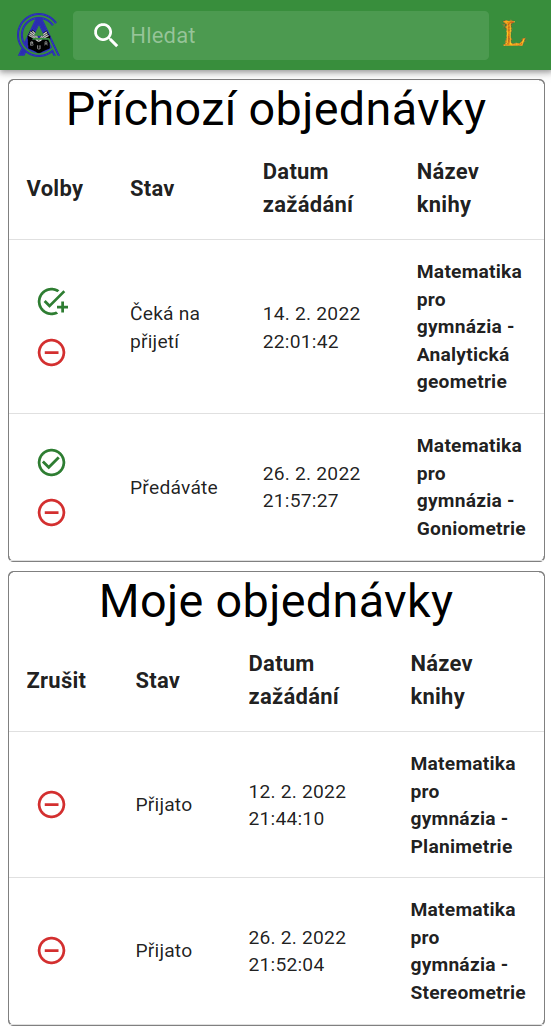
\includegraphics{../img/Requests.png}
	\vspace{-8mm}
	\caption{\textit{vrchní část profilové stránky}}\label{fig:requests}
\end{wrapfigure}

Vyžádání knihy a dále stav jednání můžeme sledovat v\,\,tabulkách na stránce našeho
profilu (\texttt{/user}). Tabulky také obsahují tlačítka s akcemi, přejetím myší
získáme podrobnější informace o akci (viz obr. \ref{fig:requests})

V žádostech o naše produkty můžeme logicky přijmout jen jednu. Proto pokud již nějaká
žádost pro danou knihu je přijata budou ostatní skryté. Až kdybychom již přijatou žádost
zrušili, třeba z důvodů příliš dlouhé domluvy, se nám zobrazí ostatní od stejné knihy.

\section{Překážky během vývoje}
První narážkou na nepříjemnosti je nejednotnost návodů a pomocných fór na internetu.
Základní balíčky Reactu (\texttt{react-router-dom}, \texttt{react-redux}...) prošli
nedávno zásadnějšími změnami, které nejsou dobře dokumentované a jejich chování může
překvapit. Jiné funkce naproti tomu nejsou konzistentí (zmiňované updatování globálního
stavu). K tomu ještě chybí znalost základů, kterých jsme měli nabýt ve třetím ročníku, a
výsledkem je program, který nemá žádné optimalizace.

\chapter*{Závěr}
\addcontentsline{toc}{chapter}{Závěr}
Program funguje, z pohledu designu je svou jednoduchostí i poměrně pěkný. Vše, co jej dělá
užitečným, už pracuje tak, jak má, a to stabilně -- s případnými záchytnými body.

Ačkoliv provozuschopnost aplikace dosáhla navrženého minima, vyskytuje se v kódu i nadále
mnoho věcí, které by stálo za to přidat, či v několika případech také zlepšit (filtrování
knih na straně klienta). Příkladem toho je navržení pro malé rozměry -- v aktuální podobě
vždy pošleme seznam všech knih v databázi, namísto posílání po částech na vyžádání.

K větším negativním vlastnostem patří scházející handlování o ceny, které lze napodobit
úpravou ceny uvedené na inzerátu, což docílí stejného efektu, ale ve většině případů
pravděpodobně nebude příliš využíváno.

Podobný dopad má skrytí kontaktních údajů do doby přijetí. Uživatel nemá možnost
komunikovat s více lidmi současně a dát knihu rychlejšímu. Na druhou stranu toto osobně
považuji za pozitivní. Vyhýbáme se tím situacím, kdy by uživatelé zbytečně marnili čas s
jedním inzerentem, zatímco takto mohou požádat u více lidí, a\,\,obchod provádět s tím,
který jako první odpoví jim. Tímto se přenáší soutěživost mezi prodávající namísto kupců,
což odpovídá mnohdy i skutečnosti.

Bonus v podobě designu pro mobilní zařízení považuji za dosažený -- Všechny ukázky z
programu byly v rozměrech telefonů a nevidím v nich chybu. Oproti tomu pohled na počítači
by mohl zužitkovat menšího zlepšení, avšak fotky beztak budou nahrávané převážně z
elektroniky vybavené fotoaparátem.

Výhodnější balíčky by určitě stály za doprogramování, ale další tabulka spolu s novým
odkazem pro zobrazení obsahu by měla cenu jen, pokud by program byl využíván.

Administrátor by do databází neměl mít potřebu zasahovat, a pokud ano, jednalo by se
pravděpodobně o stav, kdy by aplikace stejně nemohla běžet a byl by zapotřebí přímý
přístup, což prakticky eliminuje pointu správy z prostředí webové stránky.

Kdyby byla šance, že tato aplikace by běžela pod určitou doménou, stálo by za to do
budoucna implementovat i chat do stránky, aby komunikace probíhala pohodlněji. To by
bohužel znamenalo buď větší spam emailů po každé zprávě protější strany, nebo nutnost
stránku neustále kontrolovat, takže výhoda této funkce je pochybná.

\bibliographystyle{czplainnat}   %% Autor (rok) s českými spojkami
%\bibliographystyle{plainnat}    %% Autor (rok) s anglickými spojkami
%\bibliographystyle{unsrt}       %% [číslo]


\renewcommand{\bibname}{Seznam použité literatury}

\nocite{*}
\bibliography{literatura}

%%% Kdybyste chtěli bibliografii vytvářet ručně (bez bibTeXu), lze to udělat
%%% následovně. V takovém případě se řiďte normou ISO 690 a zvyklostmi v oboru.

% \begin{thebibliography}{99}
%
% \bibitem{lamport94}
%   {\sc Lamport,} Leslie.
%   \emph{\LaTeX: A Document Preparation System}.
%   2. vydání.
%   Massachusetts: Addison Wesley, 1994.
%   ISBN 0-201-52983-1.
%
% \end{thebibliography}


\listoffigures
\openright
\end{document}
